\section*{\large{ВВЕДЕНИЕ}}

Цель лабораторной работы --- разработать программу сжатия <<LZW>> \cite{Enigma}.

Задачи лабораторной работы:

\begin{enumerate}
    \item провести анализ работы сжатия <<LZW>>;
    \item описать алгоритм сжатия;
    \item релизовать описанный алгоритм.
\end{enumerate}

\clearpage
\section{Аналитическая часть}

\subsection{Алгоритм шифрования LZW}

\textbf{LZW} \cite{Enigma} --- алгоритм сжатия, основывающийся на поиске схожих символов в файле.

\subsubsection{Алгоритм:}

\textbf{Кодирование}

\begin{itemize}
	\item[---]  Все возможные символы заносятся в словарь. Во входную фразу X
  заносится первый символ сообщения.
	\item[---] Считать очередной символ Y
  из сообщения.
	\item[---] Если Y --- это символ конца сообщения, то выдать код для X, иначе:
	\item[---] Если фраза XY уже имеется в словаре, то присвоить входной фразе значение XY и перейти к Шагу 2,
	\item[---] Иначе выдать код для входной фразы X, добавить XY в словарь и присвоить входной фразе значение Y. Перейти к Шагу 2.

\end{itemize}

\textbf{Декодирование}

\begin{enumerate}
  \item[---] Все возможные символы заносятся в словарь. Во входную фразу X
  заносится первый код декодируемого сообщения.
  \item[---] Считать очередной код Y из сообщения.
  \item[---] Если Y --- это конец сообщения, то выдать символ, соответствующий коду X, иначе:
  \item[---] Если фразы под кодом XY нет в словаре, вывести фразу, соответствующую коду X, а фразу с кодом XY занести в словарь.
  \item[---] Иначе присвоить входной фразе код XY и перейти к Шагу 2.
\end{enumerate}

\clearpage

\section{Конструкторская часть}

\subsection{Разработка алгоритма}

На рисунке \ref{fig:algo} представлена схема алгоритма шифрования LZW.

%

\begin{figure}[h!]
	\centering
	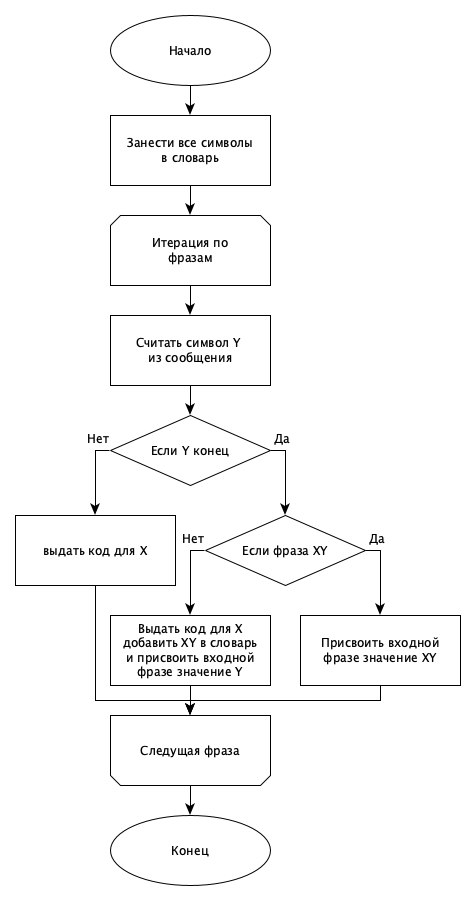
\includegraphics[width=0.5\textwidth]{assets/graphs/lzf.png}
	\caption{Схемы алгоритма LZW}
  \
	\label{fig:algo}
\end{figure}
\clearpage

\section{Технологическая часть}

\subsection{Средства реализации}

Для реализации ПО был выбран язык C++ \cite{c++}.
В данном языке есть все требующиеся инструменты для данной лабораторной работы.
В качестве среды разработки была выбрана среда VS code \cite{vscode}.

\subsection{Реализация алгоритма}

Реализация кодирования LZW.

\begin{lstlisting}
	void compressInternal(const std::vector<uint8_t>& inputFile)
	{
		initializeDictionary();

		std::vector<uint8_t> currentSubsequence;
		int nextIndex = 0;
		uint8_t nextByte;
		TrieNode* currentNode = rootNode;

		int code = 0xFF + 1;

		while (nextIndex < inputFile.size())
		{
			nextByte = inputFile[nextIndex];
			if (currentNode->children.contains(nextByte))
			{
				currentNode = &currentNode->children[nextByte];
				nextIndex++;
			}
			else
			{
				tempOut->emplace_back(currentNode->code, getBitsToRepresentInteger(code));
				currentNode->children[nextByte].code = code;
				code++;
				currentNode = rootNode;
			}
		}

		if (currentNode != rootNode)
		{
			tempOut->emplace_back(currentNode->code, getBitsToRepresentInteger(code));
		}

		std::cout << "dict size: " << getDictSize() << std::endl;
	}
\end{lstlisting}


\subsection{Тестовые данные}

В таблице \ref{tbl:functional_test} приведены тесты для алгоритма шифрования LZW. 
Применена методология черного ящика. Тесты пройдены \textit{успешно}.

\begin{table}[ht!]
	\begin{center}
		\captionsetup{justification=raggedright,singlelinecheck=off}
		\caption{\label{tbl:functional_test} Функциональные тесты}
		\begin{tabular}{|c|c|c|}
			\hline
			Входная строка & Размер входной (Байт) & Размер выходной (Байт) \\ 
			\hline
			$aba$ & $3$ & $4$ \\
			$abaaba$  & $6$ & $6$\\
			$<<>>$  & $0$ & 0\\
      $abaabaabaaba$ & $12$ & 8 \\
			\hline
		\end{tabular}
	\end{center}
\end{table}

\clearpage
\section*{\large{ЗАКЛЮЧЕНИЕ}}
В данной лабораторной работе:
\begin{enumerate}
    \item проведен анализ работы сжатия <<LZW>>;
    \item описан алгоритм сжатия;
    \item реализован описанный алгоритм;
\end{enumerate}